\subsection{Огляд користувацького інтерфейсу}
\label{subsec:interface-subsection}

Розуміння інтерфейсу має вирішальне значення, оскільки воно закладає основу для безперешкодної навігації та ефективного використання функцій програми. Цей підрозділ має на меті ознайомится з елементами інтерфейсу, їхнім призначенням і тим, як вони впливають на загальний користувацький досвід.

Завдяки детальному вивченню інтерфейсу користувачі отримають повне уявлення про візуальну ієрархію програми, навігаційні меню, функціональність пошукового рядка, відображення карти та інші інтерактивні елементи. Буде висвітлено інтуїтивно зрозумілі дизайнерські рішення, які були реалізовані для забезпечення простоти використання та швидкого доступу до основних функцій.

У підрозділі аналізу інтерфейсу також обговорюватимуться найкращі практики та поради щодо ефективної навігації та використання елементів інтерфейсу. Користувачі дізнаються, як взаємодіяти з різними компонентами, налаштовувати свої уподобання, а також користуватися комбінаціями клавіш і жестами, щоб покращити загальний досвід роботи.

Заглибившись в аналіз інтерфейсу, можна отримають можливість легко орієнтуватися в додатку і використовувати всі його можливості. Незалежно від того, чи ви новачок, чи досвідчений користувач, цей підрозділ надасть цінну інформацію для оптимізації взаємодії та спрощення процесу планування маршрутів.

Коли користувач вперше заходить на сайт, він бачить початкову сторінку. На ній відображено коротку інформацію про застосунок та кнопку для переходу до пошуку, щоб користувач міг якомога швидше знайти потрібний маршрут.

\begin{figure}[!htp]
	\centering
	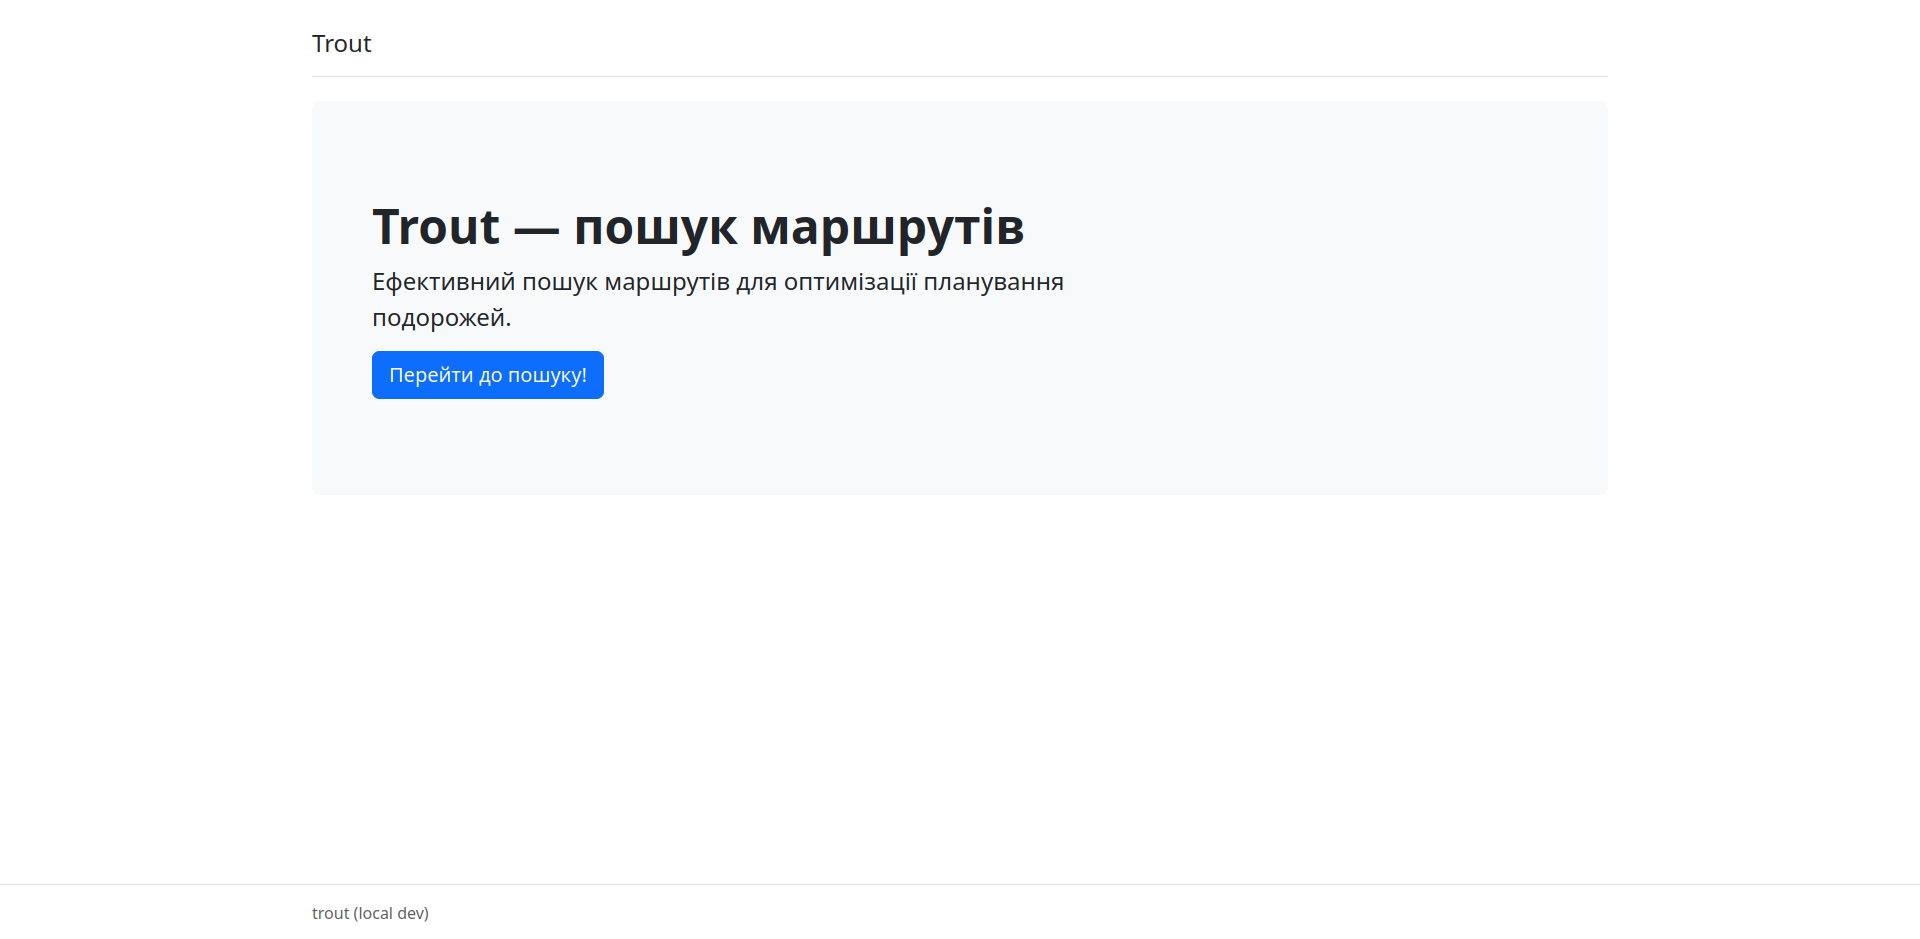
\includegraphics[scale=0.4]{content/chapters/4-results/assets/img/example_mainpage.png}
	\caption{Головна сторінка сайту}
	\label{fig:main_page}
\end{figure}

Завдяки використанню Bootstrap інтерфейс підходить для екранів будь-якого розміру

\begin{figure}[!htp]
	\centering
	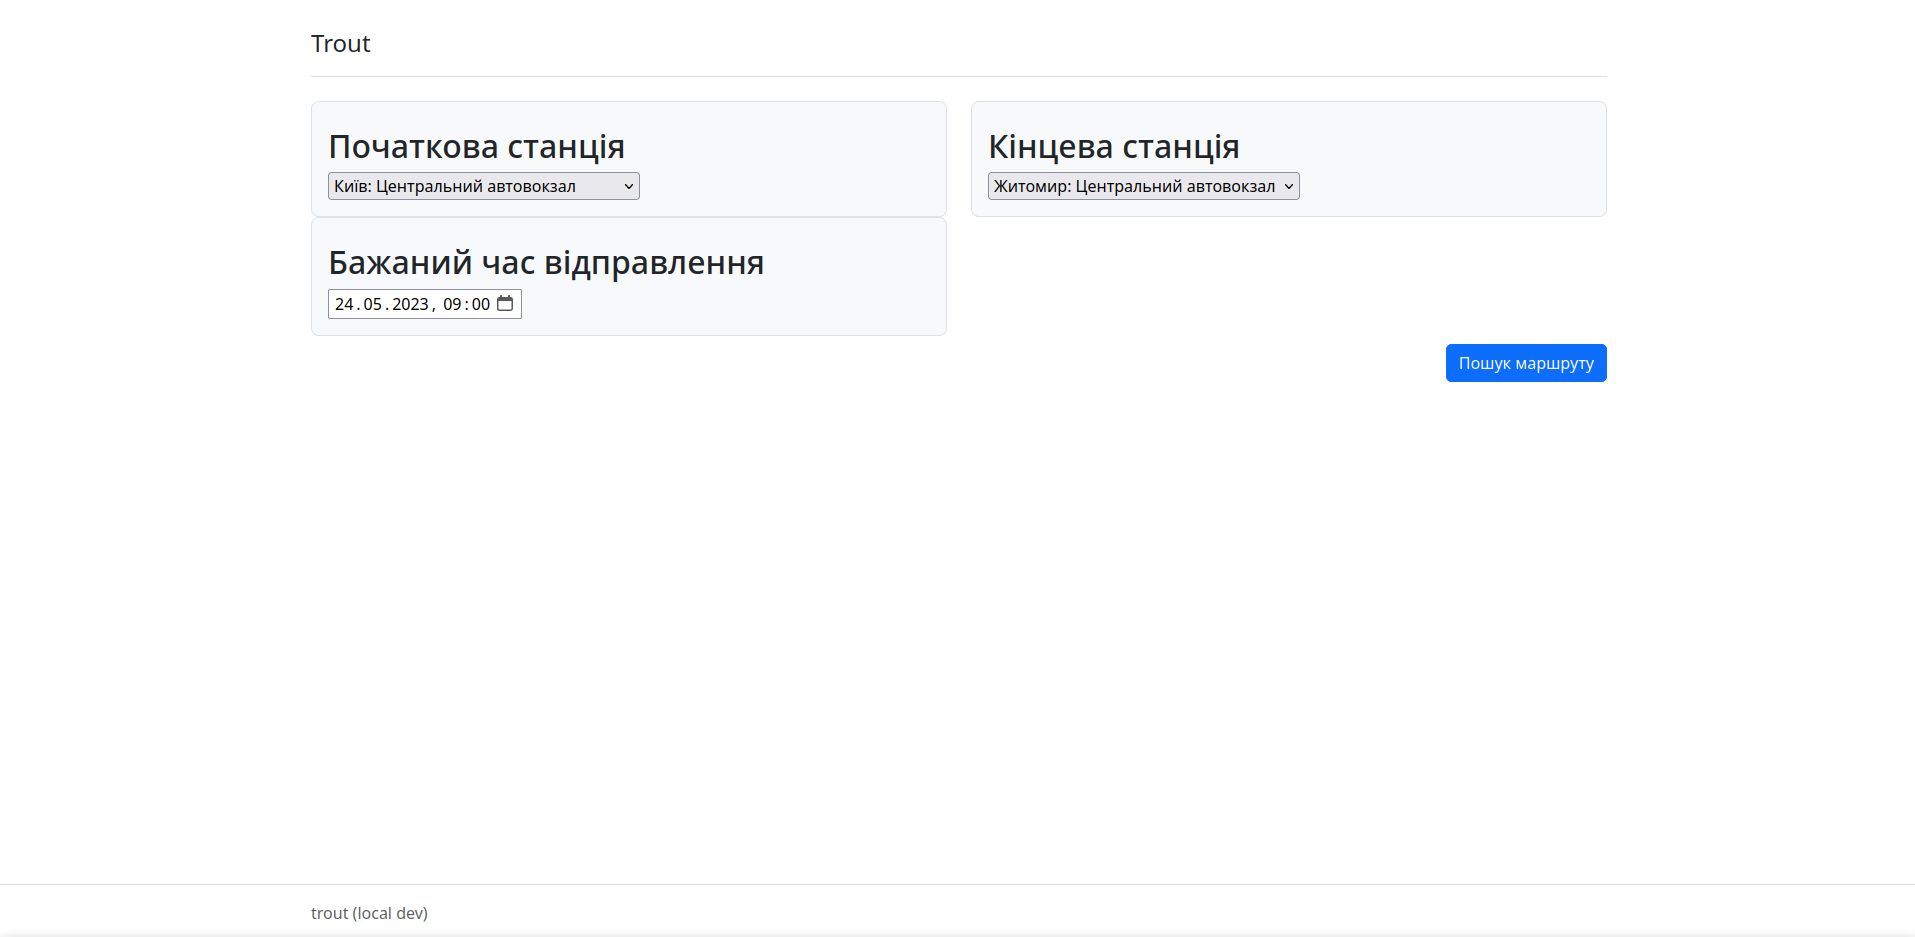
\includegraphics[scale=0.4]{content/chapters/4-results/assets/img/pc_screen.png}
	\caption{Відображення сайту на екрані комп'ютера}
	\label{fig:pc_page}
\end{figure}

\begin{figure}[!htp]
	\centering
	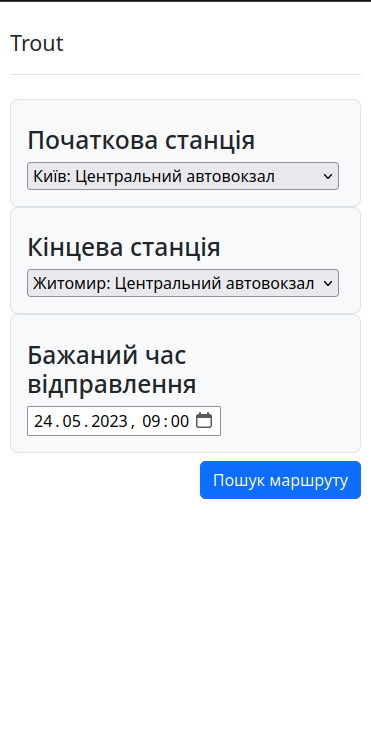
\includegraphics[scale=0.5]{content/chapters/4-results/assets/img/phone_screen.png}
	\caption{Відображення сайту на екрані телефону}
	\label{fig:phone_page}
\end{figure}
